\section{Definition of deep neural networks (DNN)} 
In this section, we will give a brief introduction to a special
function class related to deep neural networks (DNN) used in machine
learning.  We then explore the relationship between DNN (with ReLU as
activation function) and linear finite element methods. 

Given $n, m\ge 1$, the first ingredient in defining a deep neural
network (DNN) is (vector) linear functions of the form
\begin{equation}\label{thetamap1}
\theta:\mathbb{R}^{n}\to\mathbb{R}^{m} ,
\end{equation}as $\theta(x)=Wx+b$ where
$W=(w_{ij})\in\mathbb{R}^{m\times n}$, $b\in\mathbb{R}^{m}$. 
The second main ingredient is a nonlinear activation function, usually
denoted as 
\begin{equation}\label{sigma}
\sigma: \mathbb{R} \to \mathbb{R}.
\end{equation} 
By applying the function to each component, we can extend this
naturally to 
$$
\sigma:\mathbb R^{n}\mapsto \mathbb R^{n}.
$$


\subsection{Definition of neurons}
\begin{enumerate}
	\item Primary variables $n_0=d$
	$$
	x^0=x=
	\begin{pmatrix}
	x_1\\
	x_2\\
	\vdots \\  
	x_{d}
	\end{pmatrix}
	$$
	\item $n_1$ hyperplanes $\theta^{0}(x^0) = W^0 x + b^0$ where $W^0: \mathbb{R}^{d} \mapsto \mathbb{R}^{n_1}$:
	$$
	W^0x+b^0=
	\begin{pmatrix}
	w^0_1x+b^0_1\\
	w^0_2x+b^0_2\\
	\vdots \\  
	w^0_{n_1}x+b^0_{n_1}
	\end{pmatrix}\quad \mbox{with }\quad W^0=
	\begin{pmatrix}
	w^0_1\\
	w^0_2\\
	\vdots \\  
	w^0_{n_1}
	\end{pmatrix},\quad b^0=
	\begin{pmatrix}
	b^0_1\\
	b^0_2\\
	\vdots \\  
	b^0_{n_1}
	\end{pmatrix}
	$$
	\item $n_1$-neurons:
	$$
	x^1=\sigma(W^0x+b^0)
	=\begin{pmatrix}
	\sigma(w^0_1x+b^0_1)\\
	\sigma(w^0_2x+b^0_2)\\
	\vdots \\  
	\sigma(w^0_{n_1}x+b^0_{n_1})
	\end{pmatrix}
	$$
%	\begin{center}
%	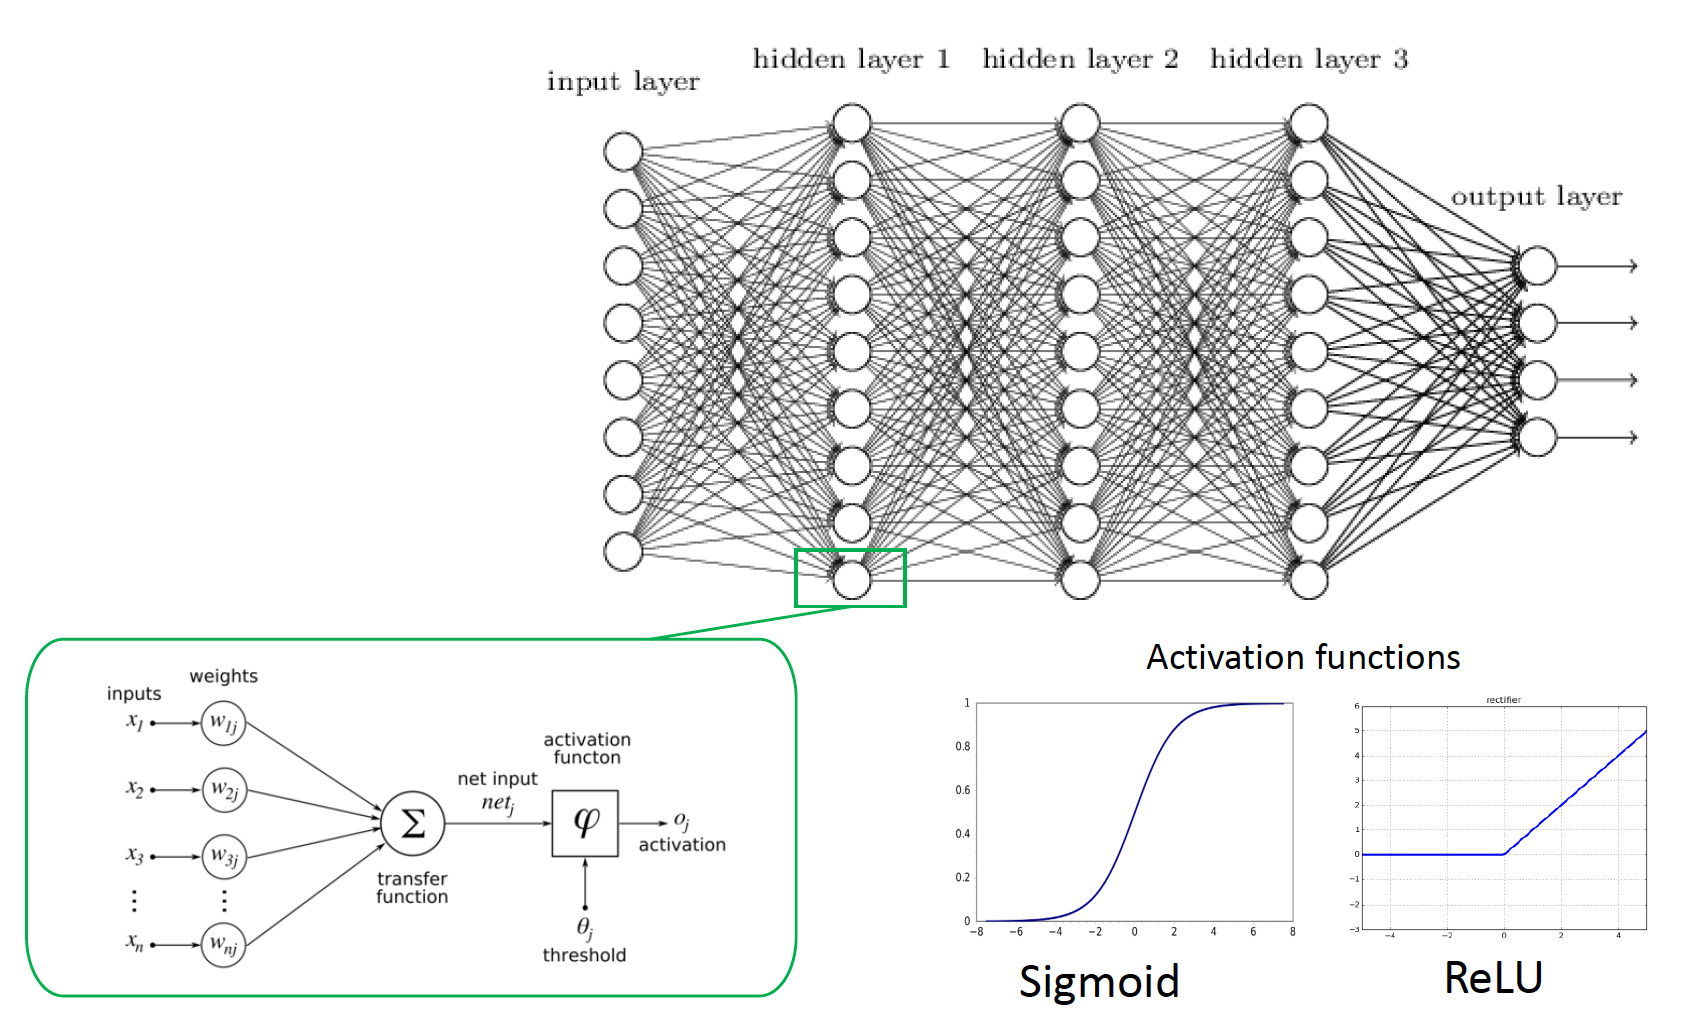
\includegraphics[height=.5\textwidth]{ANN}
%	\end{center}
	
	\item $n_2$-hyperplanes $\theta^{1}(x^1) = W^1 x + b^1$ where $W^1: \mathbb{R}^{n_1} \mapsto \mathbb{R}^{n_2}$:
	$$
	W^1x^1+b^1=
	\begin{pmatrix}
	w^1_1x^1+b^1_1\\
	w^1_2x^1+b^1_2\\
	\vdots \\  
	w^1_{n_2}x^1+b^1_{n_2}
	\end{pmatrix}\quad \mbox{with }\quad 
	W^1=
	\begin{pmatrix}
	w^1_1 \\
	w^1_2 \\
	\vdots \\  
	w^1_{n_2} 
	\end{pmatrix},\ 
	b^1=
	\begin{pmatrix}
	b^1_1\\
	b^1_2\\
	\vdots \\  
	b^1_{n_2}
	\end{pmatrix}
	$$
	\item $n_2$-neurons:
	$$
	x^2=\sigma(W^1x+b^1)
	=\begin{pmatrix}
	\sigma(w^1_1x+b^1_1)\\
	\sigma(w^1_2x+b^1_2)\\
	\vdots \\  
	\sigma(w^1_{n_2}x+b^1_{n_2})
	\end{pmatrix}
	$$
	\item $\cdots$
\end{enumerate} 

\subsection{Definition of deep neural network functions}\label{sec:DNN}
Given $d, k\in\mathbb{N}^+$ and  
$$
n_1,\dots,n_{k}\in\mathbb{N} \mbox{ with }n_0=d, n_{k+1}=1, 
$$
a general DNN function from $\mathbb{R}^d$ to $\mathbb{R}$ is given by
\begin{align*}
f^0(x)   &=\theta^0(x) \\ 
f^{\ell}(x) &= [  \theta^{\ell} \circ \sigma ](f^{\ell-1}(x)) \quad \ell = 1:k \\
f(x) &= f^k(x). 
\end{align*}
The following more concise notation is often used in computer science literature:
\begin{equation}
\label{compress-dnn}
f(x) = \theta^{k}\circ \sigma \circ \theta^{k-1} \circ \sigma \cdots \circ \theta^1 \circ \sigma \circ \theta^0(x),
\end{equation}
here $\theta^i: \mathbb{R}^{n_{i}}\to\mathbb{R}^{n_{i+1}}$ are linear
functions as defined in \eqref{thetamap1}.  Such a DNN is called a
$(k+1)$-layer DNN, and is said to have $k$-hidden layers. The size of
this DNN is $n_1+\cdots+n_k$.

Thus, we have the following connection of neurons and DNN functions
$$
f^k(x) = \theta^{k}(x^k) = \theta^{k} \circ \sigma \circ \theta^{k-1}(x^{k-1}) = [\theta^{k} \circ \sigma ] (f^{k-1}),
$$
or we can see that
$$
x^k = \sigma(f^{k-1}) = \sigma \circ \theta^{k-1} \circ \sigma (f^{k-2}) = [\sigma \circ \theta^{k-1}] (x^{k-1}).
$$
Based on these notation and connections, we have the following definition of
general artificial neural network functions.

Shallow (one hidden layer) neural network functions:
\begin{equation}
\label{NN1}
\dnn(\sigma; n_1) 
=\bigg\{ f^1(x) = \theta^1 (x^1), \mbox{ with } W^\ell\in \mathbb R^{n_{\ell+1}\times
	n_{\ell}}, b^\ell\in\mathbb R^{n_\ell}, \ell=0, 1, n_0=d, n_2 = 1\bigg\}  
\end{equation}
Deep neural network functions:
\begin{equation}
\label{NNL}
\dnn(\sigma; n_1,n_2,\ldots, n_L)=\bigg\{ f^{L}(x) = \theta^L (x^{L}), 
 \mbox{ with } W^\ell\in \mathbb R^{n_{\ell+1}\times
	n_{\ell}}, b^\ell\in\mathbb R^{n_\ell}, \ell=0:L, n_0=d, n_{L+1}=1\bigg\}  
\end{equation}
If we ignore the width (number of neurons) of network functions, we may 
denote the general deep neural network functions with certain layers.

The 1-hidden layer (shallow) neural network is defined as:
\begin{equation}
\dnn=\dnn(\sigma) = \dnn^1(\sigma)
=\bigcup_{n_1\ge 1} \dnn(\sigma;n_1,1)
\end{equation}
Generally, we can define the L-hidden layer neural network as:
\begin{equation}
\dnn^L(\sigma) := \bigcup_{n_1, n_2, \cdots, n_{L}\ge 1} \dnn(\sigma;n_1,n_2,\cdots,n_L, 1).
\end{equation}







\subsection{ReLU DNN}
In this section, we mainly consider a special activation function,
known as the {\it rectified linear unit} (ReLU), and defined as $\rm
ReLU: \mathbb R\mapsto \mathbb R$,
\begin{equation}
\label{relu}
 {\rm ReLU}(x):=\max(0,x), \quad x\in\mathbb{R}. 
\end{equation}
A ReLU DNN with $k$ hidden layers might be written as:
\begin{equation}
\label{relu-dnn}
f(x) = \theta^{k}\circ {\rm ReLU} \circ \theta^{k-1} \circ {\rm ReLU} \cdots \circ \theta^1 \circ {\rm ReLU} \circ \theta^0(x).
\end{equation}

We note that $\rm ReLU$ is a continuous piecewise linear (CPWL) function.
Since the composition of two CPWL functions is still a CPWL
function, we have the following observation~\cite{arora2016understanding}.
\begin{lemma}\label{dnn-cpwl}
	Every ReLU DNN: $\mathbb{R}^d\to\mathbb{R}^c$ is a continuous
	piecewise linear function.  More specifically, given any ReLU DNN,
	there is a polyhedral decomposition of $\mathbb R^d$ such that this
	ReLU DNN is linear on each polyhedron in such a decomposition.
\end{lemma}

Here is a simple example for the ``grid" created by some 2-layer ReLU DNNs in $\mathbb{R}^2$.

\begin{figure}[ht]
	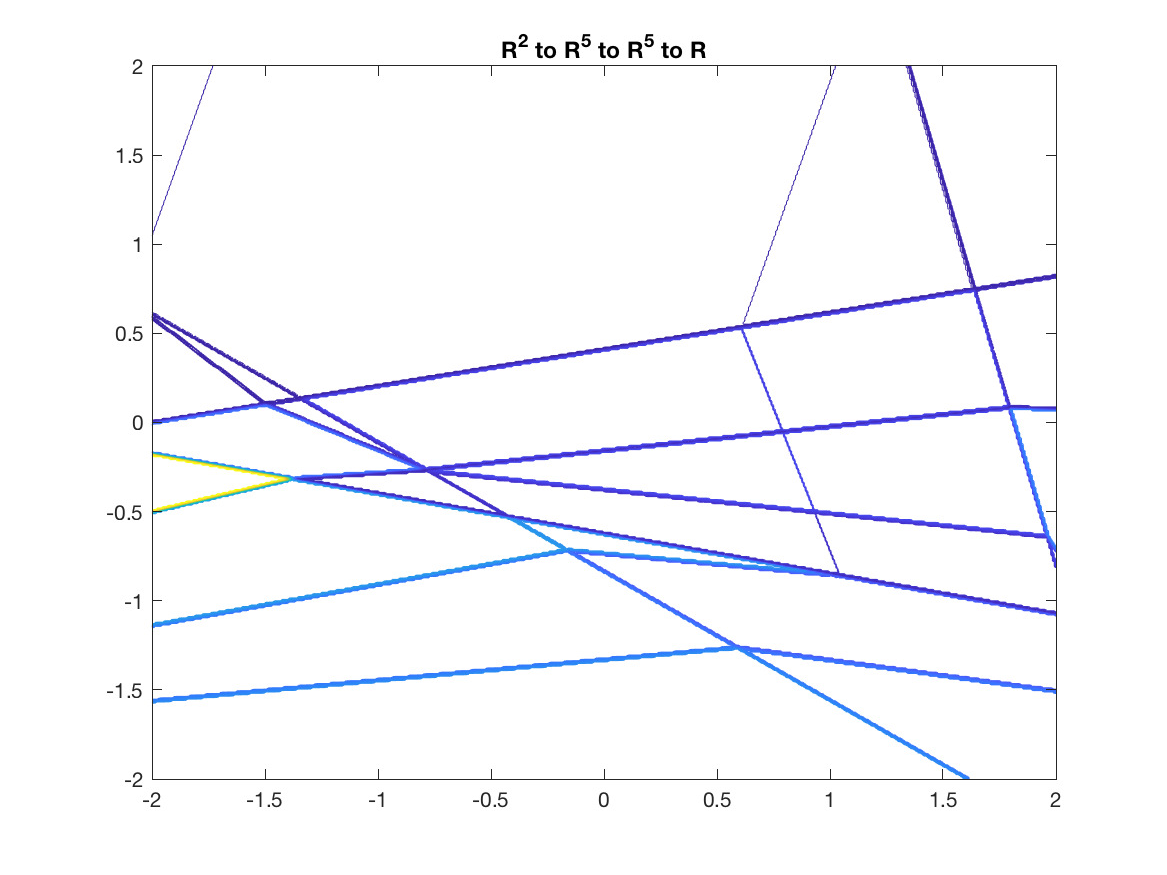
\includegraphics[width=.3\textwidth]{figures/2to5to5to1-eps-converted-to.pdf}  
	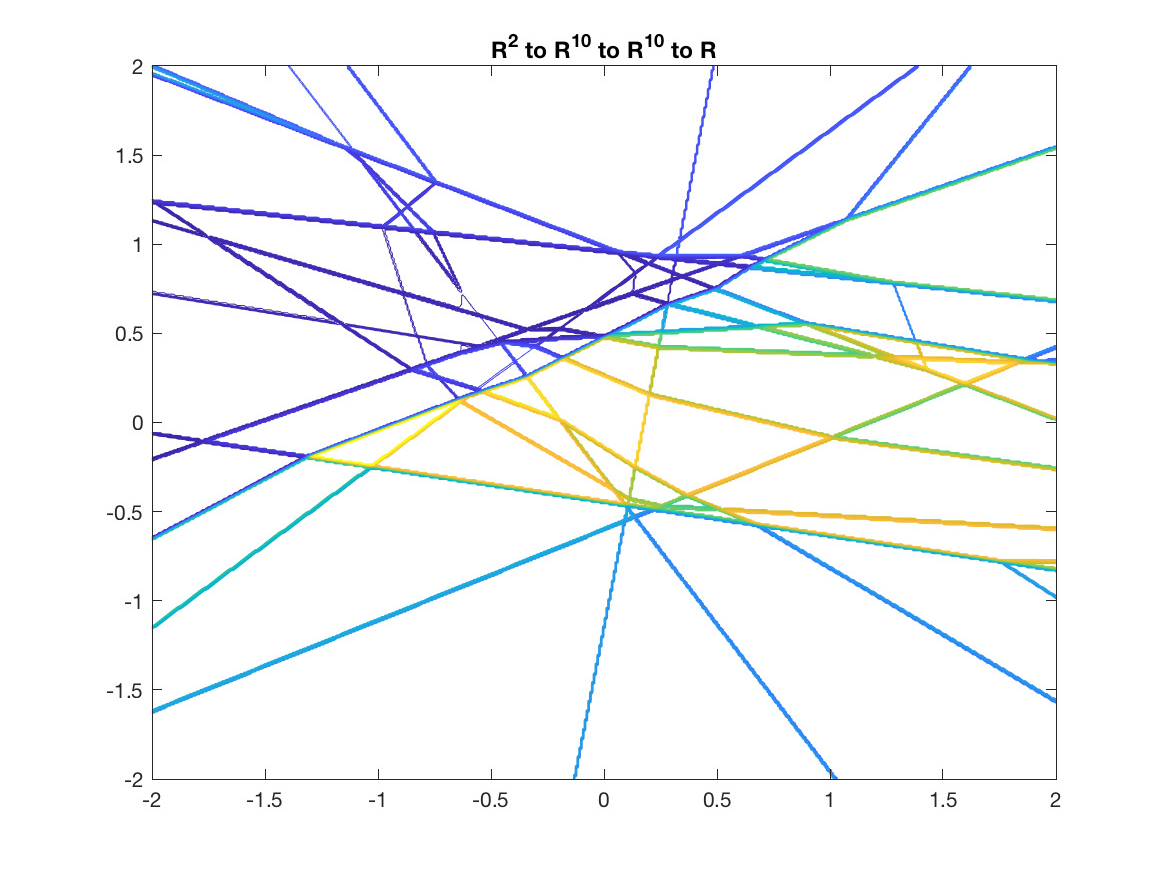
\includegraphics[width=.3\textwidth]{figures/2to10to10to1-eps-converted-to.pdf}  
	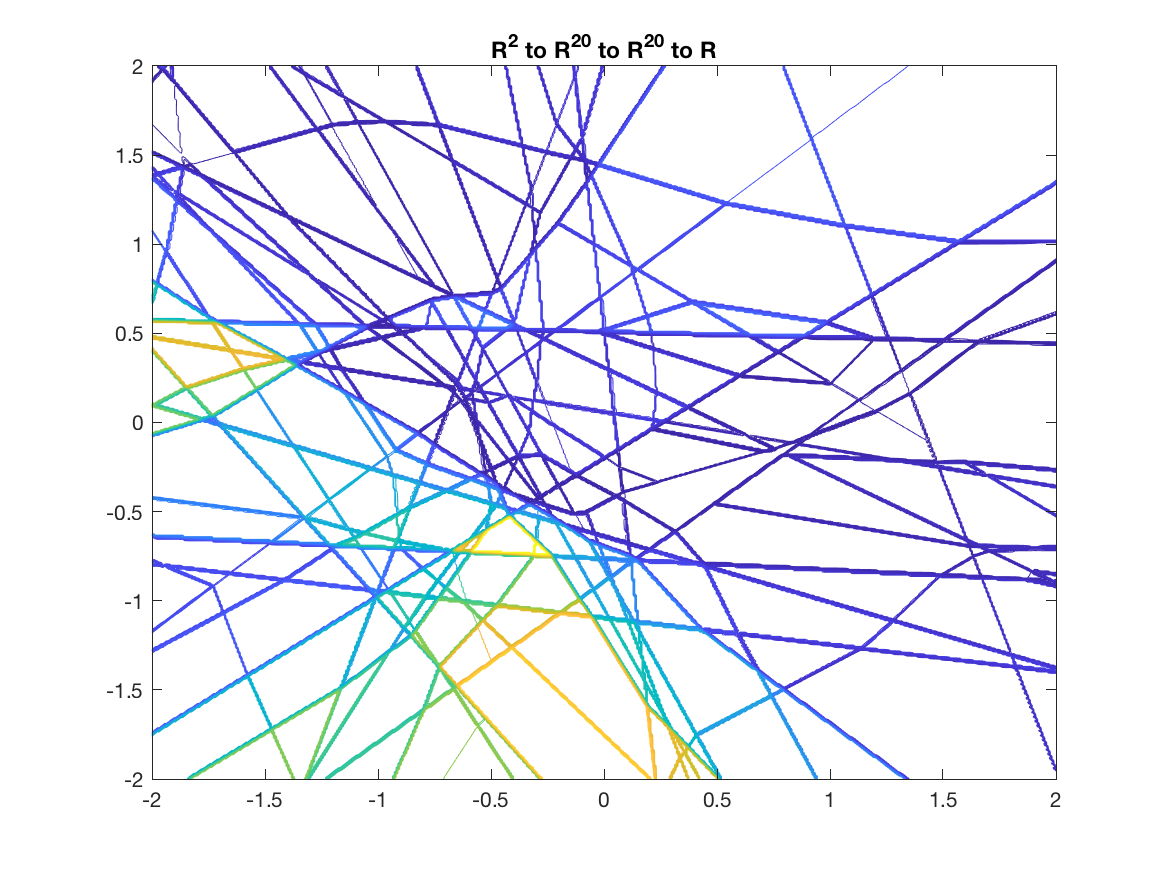
\includegraphics[width=.3\textwidth]{figures/2to20to20to1-eps-converted-to.pdf}  
	\caption{Projections of the domain partitions formed by 2-layer ReLU DNNs with sizes $(n_0, n_1, n_2, n_3)= (2, 5, 5, 1), (2, 10, 10, 1) \text{and}\ (2, 20, 20, 1)$ with random parameters.}
	\label{fig:dnn-region}
\end{figure}

For convenience of exposition,  we introduce the following notation:
%\begin{equation}
%\begin{aligned}
%{\rm{DNN}_L} :=\{& f:f=
%\theta^L \circ {\rm ReLU} \circ \theta^{L-1} \cdots {\rm ReLU}\circ \theta^0(x), \\
%&\theta^\ell \in \mathbb{R}^{n_{\ell} \times (n_\ell+1)}, \quad n^0 = d, \quad n^{L+1} = 1, \quad n^\ell \in \mathbb{N}^+\}.
%\end{aligned}
%\end{equation}
Namely $\dnn^L({\sigma})$ represents the DNN model with $L$ hidden layers and
ReLU activation function with arbitrary size, if $\sigma = {\rm ReLU}$.

